\documentclass{article}

\usepackage[ngerman]{babel}
\usepackage[utf8x]{inputenc}
\usepackage[T1]{fontenc}
\usepackage{lmodern}
\usepackage{graphicx} 
\usepackage{subfigure}
\usepackage{wrapfig}
\usepackage{adjustbox}
\usepackage{caption}
\usepackage{enumitem}
\usepackage {ulem}
%\usepackage{algorithmic}
\usepackage{algpseudocode}
\usepackage{geometry}
\geometry{a4paper, left=2.5cm, right=2.5cm, top=2.5cm, bottom=3cm}

\title{Bachelorarbeit\\
	Algorithmische Lösung des Potenzial-Problems\\
	auf Grundlage des Papers:\\
	"Capture of an Indruder by Mobile Agents"}
\author{Jens Harder}
\date{\today}


\begin{document}
	\maketitle
	\newpage
	
	\pagenumbering{arabic}.
	\tableofcontents
	
	\newpage
	
	\section{Einleitung}
Diese Bachelorarbeit ist aus einer Projektarbeit entstanden, welche im Semester 2014/15 stattgefunden hat.\\

In dieser Projektarbeit habe ich einen Algorithmus aus dem Paper "'Capture of an Intruder by Mobile Agents"' (BARRIÈRE L. et al. 2002) in einem Java-Applet visuell dargestellt und implementiert. Es handelt sich bei dem Algorithmus um eine Variante des sogenannten "'graph-searching problems"'.\\

Man kann sich das Problem anschaulich wie folgt vorstellen: Ein Einbrecher ist in das Netzwerk eingedrungen und soll nun von mobilen Agenten gesucht werden. Sowohl die Agenten, als auch der Einbrecher können sich nur auf den Kanten des Graphen bewegen. Der Algorithmus soll die minimale Anzahl der Agenten berechnen, sowie den Knoten angeben, wo die Agenten die Suche im Baum anfangen sollen (die sogenannte Homebase), ohne zu wissen, wo sich der Einbrecher befindet. Je nachdem welcher Knoten als Homebase ausgewählt wird, kann sich die benötigte Anzahl an Agenten evt. ändern.\\

Da dieses Problem NP-Vollständig auf auf allgemeinen Graphen ist, werden sowohl im Paper, als auch in dieser Bachelorarbeit, nur Bäume betrachtet. Dadurch ist es möglich, einen linearen Algorithmus anzugeben, in dem die minimale Anzahl an Agenten sowie die dazugehörige Homebase berechnet werden.\\

Eine wichtige Eigenschaft, die wir aufrecht erhalten wollen ist die Monotonie. Diese bedeutet in diesem Fall, dass ein Knoten, den wir bereits dekontaminiert haben (kontrolliert, dass der Einbrecher dort nicht ist), nicht mehr kontaminiert werden kann (der Einbrecher bekommt keine Möglichkeit mehr in diesen Knoten zu gelangen). Um diese Eigenschaft zu gewährleisten müssen wir sogenannte Wachen aufstellen, die dekontaminierte Teilbäume vor dem Einbrecher schützen. Die einzelnen Teilbäume werden von den Agenten sukzessive kontrolliert, bis wir den ganzen Baum dekontaminiert haben.\\
\\
\\

Das Ziel dieser Bachelorarbeit ist es, auf Grundlage des in "'Capture of an Intruder by Mobile Agents"' (BARRIÈRE L. et al. 2002) beschriebenen Algorithmus weitere Problemstellungen zu betrachten. Ich untersuche im folgenden, wie sich ein Potenzial auf den Algorithmus auswirkt. Das Potenzial gibt an, um wieviel eine oder mehrere Kanten(-gewichte) reduziert werden können. Der Algorithmus soll in der Lage sein, dieses Potenzial zu nutzen, um die minimale Anzahl an Agenten, die gebraucht werden, um den ganzen Baum zu dekontaminieren, zu denken. Je nachdem, welche Kanten durch das Potenzial reduziert werden, ändert sich die minimale Anzahl der Agenten unterschiedliche stark. Es sollen nun eine optimale Verteilung an Kanten angegeben werden, um die Agentenzahl möglichst stark zu reduzieren.\\



	
	\section{Der Algorithmus}
Im folgen werde ich zunächst den Algorithmus aus dem Paper beschreiben und erklären, sowie im Anschluss ein paar Modifikationen erläutern, mit denen ich in dieser Bachelorarbeit weiterarbeiten werde.



\subsection{Originaler Algorithmus aus dem Paper}\label{paperAlgoChapter}
Um die Anzahl der Agenten zu ermitteln, schicken sich die Baumknoten gegenseitig Nachrichten, mit der Information, wie viele Agenten mindestens benötigt werden, um einen bestimmten Teilbaum zu dekontaminieren.

%\subsubsection*{Berechnung der Nachrichten}

Als erstes berechnet der Algorithmus alle von allen Knoten ihre Knotengewichte. Dieses ergibt sich jeweils aus dem maximalen Kantengewicht aller zu diesem Knoten führenden Kanten. Also für das Knotengewicht vom Knoten x gilt: $\omega(x) = max_{e} \omega(e)$, für jede Kante e inzident zu x.
\\
\\
Nun werden die Nachrichten versendet, für die es zwei Fälle gibt:

\begin{enumerate}
			
	\item Fall: \label{paperAlgoFall1}
	
		\begin{enumerate}
			
			\item Der aktuelle Knoten x hat bereits schon mindestens n-1 Nachrichten erhalten, wobei n die Anzahl der inzidenten Knoten ist
			\\
			
				\begin{minipage}{0.50\textwidth} 
					
					Um eine Nachricht an den Nachbarknoten y zu senden, der bis zu diesem Zeitpunkt noch keine Nachricht an x gesendet hat, nimmt man die 2 größten Nachrichten ($l_{1}$ und $l_{2}$) die bei x angekommen sind. Mit diesen beiden angekommenen Nachrichten $l_{1} \ge l_{2}$ sowie dem Knotengewicht $\omega(x)$ wird die Nachricht $\lambda_{y}$ an y wie folgt berechnet:\\
					$\lambda_{y} = max\{l_{1},  l_{2} + \omega(x)\}$
					\\
					\\	
					Nach dem Berechnen und Versenden der Nachricht $\lambda_{y}$ muss x auf die letzte ankommende Nachricht (von y) warten. Sobald diese Nachricht angekommen ist, berechnet x die Nachrichten für alle anderen Nachbarknoten, wie im Fall \ref{labelAufUnterfall} beschrieben. 
				\end{minipage}
				\hfill
				\begin{minipage}{0.35\textwidth}
					
					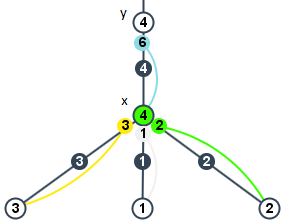
\includegraphics[width=\textwidth]{bilder/abb_paper_n-1knoten.png}
					\captionof{figure}{Die neue Nachricht (blau) von Knoten x zu Knoten y ist 6, da $l_{2} + \omega(x)$ (grün) größer ist als $l_{1}$ (gelb).}
				\end{minipage}
				
				
			\item Der aktuelle Knoten x hat bereits von allen n zu ihm inzidenten Knoten eine Nachricht erhalten, selber jedoch noch nicht zu allen Knoten eine Nachricht gesendet. Diese Nachrichten müssen nun berechnet und versendet werden:\label{labelAufUnterfall}
			\\
				
				\begin{minipage}{0.50\textwidth} 
					
					Um eine Nachricht an einen Nachbarknoten y zu senden, der bis zu diesem Zeitpunkt noch keine Nachricht von x erhalten hat, nimmt man die 2 größten Nachrichten ($l_{1}$ und $l_{2}$) die bei x angekommen. Dabei ist es wichtig, dass weder $l_{1}$ noch $l_{2}$ von y stammen. Die Nachricht von y wird bei dieser Nachrichtenberechnung ignoriert! Mit den beiden ermittelten Nachrichten $l_{1} \ge l_{2}$ sowie dem Knotengewicht $\omega(x)$ wird die Nachricht $\lambda_{y}$ an y wie folgt berechnet:\\
					$\lambda_{y} = max\{l_{1},  l_{2} + \omega(x)\}$
					\\
					\\
					Diese Berechnung wird für jeden Nachbarknoten von x wiederholt, sodass jeder Nachbar eine Nachricht von x erhält. Nach diesem Schritt ist der Knoten x mit dem Algorithmus fertig, da er sowohl von jedem Nachbar eine Nachricht erhalten hat, als auch an jeden Nachbar eine Nachricht gesendet hat.
				\end{minipage}
				\hfill
				\begin{minipage}{0.35\textwidth}
					
					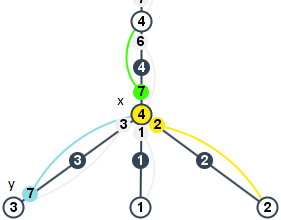
\includegraphics[width=\textwidth]{bilder/abb_paper_nknoten.png}
					\captionof{figure}{Die neue Nachricht (blau) von Knoten x zu Knoten y ist 7, da $l_{1}$ (grün) größer ist als $l_{2} + \omega(x)$ (gelb).}
				\end{minipage}
			
		\end{enumerate}
		
	\item Fall:
		
		\begin{minipage}{0.55\textwidth} 
			Zu beginn des Algorithmus, oder wenn der andere Fall nicht mehr auftritt, sendet ein beliebiger Blattknoten seine Nachricht an den eigenen Nachbarn.\\
			
			Die zu sendende Nachricht $\lambda_{y}$ vom Blatt x an seinen Nachbarknoten y ist dabei nur das eigene Gewicht:\\
			$\lambda_{y} = \omega(x)$
		\end{minipage}
		\hfill
		\begin{minipage}{0.35\textwidth}
						
			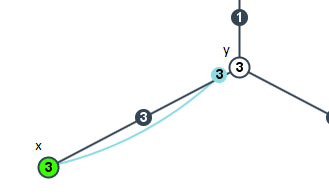
\includegraphics[width=\textwidth]{bilder/abb_blattknoten.png}
			\captionof{figure}{Das Knotengewicht des Blattknotens x (grün) bestimmt die Nachricht (blau) zum Nachbarknoten y.}
		\end{minipage}
		
\end{enumerate}

%\subsubsection*{Berechnung der minimalen Agenten}

Sobald alle Knoten sowohl an alle Nachbarn eine Nachricht geschickt haben, als auch von allen Nachbarn eine Nachricht erhalten haben (jede Kante im gesamten Baum überträgt genau 2 Nachrichten), hat jeder Knoten alle Informationen die er gebraucht werden, um die minimale Anzahl an Agenten zu errechnen, die an diesem Knoten benötigt werden:
\\
Die minimale Agentenanzahl $\mu(x)$, die am Knoten x benötigt werden, wenn dieser als Homebase definiert wird, wird wie folgt berechnet:
\\
$\mu(x) = max\{l_{1},  l_{2} + \omega(x)\}$, wobei analog zu der Berechnung der Nachrichten gilt: $l_{1} \ge l_{2}$ sind die größten beiden angekommenen Nachrichten und $\omega(x)$ ist das Knotengewicht von x.
\\
\\
Nachdem alle Knoten ihr $\mu$ berechnet haben, wird ein Knoten mit minimalen $\mu$ ausgewählt. Dieser ist die neue Homebase, von dem aus $\mu$ viele Agenten den gesamten Baum dekontaminieren können, ohne die Monotonie-Eigenschaft zu verletzen (siehe oben).



\subsection{Modifikationen am Algorithmus}


	\begin{wrapfigure}{l}{0.35\textwidth}
		\begin{center}
			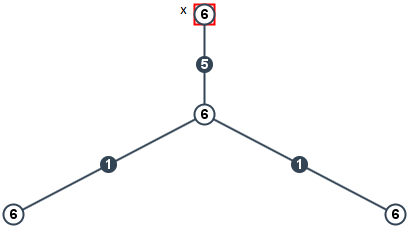
\includegraphics[width=0.35\textwidth]{bilder/abb_paper_problem.png}
		\end{center}
		\caption{Problem mit dem Algorithmus aus dem Paper. Der Knoten x sollte intuitiv mit 5 Agenten auskommen}
		\label{fig:negBeispielPaperAlgo}
	\end{wrapfigure}

Die Ergebnisse des im Paper beschriebene Algorithmus stimmt in einigen Fällen nicht mit der Intuition überein, die man bekommt wenn man einige Beispielbäume betrachtet (z.B. Abbildung \ref{fig:negBeispielPaperAlgo}). In dem  angegebenen Beispiel sollte der Knoten x mit 5 Agenten auskommen: Alle 5 Agenten gehen über die erste Kante zum mittleren Knoten. Von dort aus werden nur noch 2 Agenten benötigt: Einer hält Wache um die Monotonie zu gewährleisten und der zweite dekontaminiert ein Blatt. Zum Schluss wird das letzte Blatt von einem Agenten dekontaminiert und der Algorithmus ist fertig.
\\
Der Unterschied zwischen dem originalen Algorithmus und der Intuition ist folgender: Der originale Algorithmus plant im Beispiel für den mittleren Knoten 5 Wachen ein (das Knotengewicht ist 5), obwohl wir über die Kante mit Gewicht 5 kommen, diese dadurch dekontaminiert ist und wir sie nicht mehr bewachen müssen. Es werden dadurch mehr Agenten eingeplant, als wirklich benötigt werden.
\\
Da das Problem wie beschrieben am Knotengewicht liegt, werde ich im folgenden eine Variante des Algorithmus beschreiben, die etwas anders mit dem Knotengewicht umgeht. Allerdings kommt es zu Fehlern, wenn man nur das Knotengewicht verändert, weshalb man zusätzliche Fälle in den Algorithmus einbauen muss, damit dieser sowohl richtig, als auch intuitiv sinnvoll funktioniert:
\\
\\
Im Gegensatz zum originalen Algorithmus wird im modifizierten Algorithmus nicht mehr das Knotengewicht in die direkte Berechnung der Nachricht miteinbezogen, sondern dient nur noch dazu zu überprüfen, dass die berechnete Nachricht nicht zu klein ist.
\\
Dazu muss der Algorithmus in Kapitel \ref{paperAlgoChapter} Fall \ref{paperAlgoFall1} wie folgt abgeändert werden:

\subsubsection*{Modifizierte Berechnung der Nachricht:}

\begin{itemize}
	
	\item 
		Um eine Nachricht an einen Nachbarknoten y zu senden, der bis zu diesem Zeitpunkt noch keine Nachricht von x erhalten hat, nimmt man das Kantengewicht der zwei größten Kanten ($edge_{1}$ und $edge_{2}$) die inzident zu x sind, jedoch nicht zu y. Mit den beiden ermittelten Kantengewichten, für die gilt $edge_{1} \ge edge_{2}$ wird die Nachricht $\lambda_{y}$ an y wie auch in Abbildung \ref{modifiziert_a} gezeigt berechnet:\\
		$\lambda_{y} = edge_{1} + edge_{2}$.
		\\
		\\
		Vor der Bestimmung der zwei maximalen Kanten werden $edge_{1}$ und $edge_{2}$ auf 0 initialisiert, sodass die Berechnung auch klappt, falls es weniger als zwei Kanten gibt, auf die die Bedingung inzident zu x und nicht inzident zu y  zutrifft.
	
	\item
		Nachdem die neue Nachricht $\lambda_{y}$ nun berechnet wurde, müssen wir noch überprüfen, dass $\lambda_{y}$ nicht kleiner ist als das Knotengewicht $\omega(x)$. Ist dies der Fall bedeutet dass, dass das Kantengewicht der Kante, über die wir die Nachricht nach y schicken größer ist als die berechnete Nachricht. Da dies nicht sein darf, da wir sonst nicht genug Agenten haben würden, um über die Kante zu laufen, müssen wir die Nachricht die wir an y schicken entsprechend anpssen (Beispiel in Abbildung \ref{modifiziert_b}):
		
		\begin{algorithmic}
			\If {$\lambda_{y} < \omega(x)$}
			\State $\lambda_{y} \gets \omega(x)$
			\EndIf
		\end{algorithmic}
	
	\item
		Außerdem darf die berechnete Nachricht $\lambda_{y}$ nicht kleiner sein als die größte in x angekommene Nachricht $l_{1}$ (außer der Nachricht, die wir evt. schon von y erhalten haben). Ist die Nachricht $\lambda_{y}$ kleiner als $\l_{1}$, würden wir nicht genug Agenten bekommen, um den Teilbaum, aus dem $l_{1}$ kommt zu dekontaminieren. Wir müssen $\lambda_{y}$ kontrollieren und evt. wie in Abbildung \ref{modifiziert_c} anpassen:
		
		\begin{algorithmic}
			\If {$\lambda_{y} < l_{1}$}
			\State $\lambda_{y} \gets l_{1}$
			\EndIf
		\end{algorithmic}
	
\end{itemize}

\begin{figure}[h]
	\subfigure[Die Nachricht $\lambda_{y}$ (blau) von x zu y ist 5, da $edge_{1}$ und $edge_{2}$ (beide grün) die entscheidenden Kanten sind. y.\label{modifiziert_a}]{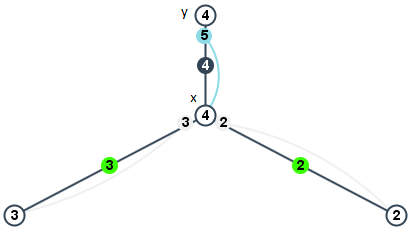
\includegraphics[width=0.32\textwidth]{bilder/abb_neu_max1max2.png}}
	\hfill
	\subfigure[Da das Knotengewicht durch die Kante zwischen x und y bestimmt wird (grün) und dieses größer ist als die Summe der beiden normalen Kanten $edge_{1}$ und $edge_{2}$ (gelb), bestimmt diese Kante die Nachricht $\lambda_{y}$ (blau). \label{modifiziert_b}]{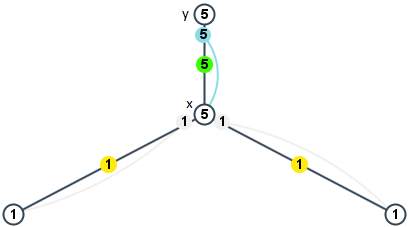
\includegraphics[width=0.32\textwidth]{bilder/abb_neu_edge.png}} 
	\hfill
	\subfigure[Die größte Nachricht (grün), die an x ankommt ist größer als die beiden Kanten $edge_{1}$ und $edge_{2}$ (gelb) und bestimmt dadurch die die Nachricht $\lambda_{y}$ (blau). \label{modifiziert_c}]{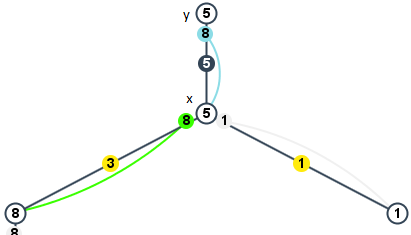
\includegraphics[width=0.32\textwidth]{bilder/abb_neu_msgData.png}}  
	
	\caption{Drei Fälle, die bei der Modifizierung des Algorithmus beachtet werden müssen, um alle Spezialfälle abzudecken.} 
\end{figure} 





	\section{Das Potenzial-Problem}

\subsection{Spezialfall k = 1}
//algo angeben, wieso ist er liniear? wieso korrekt?\\


Die Idee des Algorithmus ist es, zu protokollieren, welche Kante(n) für welche Knoten von Bedeutung ist:\\

Jeder Knoten berechnet im Algorithmus von BARRIÈRE L. et al. die minimale Anzahl von Agenten und jede Knoten hat mindestens eine Kante von der seine Agentenanzahl von abhängt.

\subsection{Potenzial auf einer Kante mit k > 1}

Um das Problem des Potenzials etwas zu erweitern, betrachte ich im folgenden Abschnitt Potenziale größer 1, allerdings mit der Einschränkung, dass man das gesamte Potenzial k nur auf einer Kante einsetzen darf.

Es fällt zunächst auf, dass man nicht garantieren kann, dass sich die Anzahl der benötigten Agenten auf allen Bäumen reduzieren lässt. Hierbei spielt es auch keine Rolle, wie groß das Potenzial k ist, da allein die Eigenschaft, dass man das Potenzial nur auf einer Kante einsetzen kann, genügt, um ein Gegenbeispiel zu finden:

Da das Potenzial k beliebig groß ist, kann man eine Kante auf Kantengewicht 1 setzen, man dadurch das größtmögliche Potenzial ausnutzt. Trotzdem ist es nicht möglich bei folgendem Baum die Anzahl der Agenten zu reduzieren:

\begin{figure}[h]
	\subfigure[alle Kanten haben Gewicht 4. Alle Knoten benötigen mindestens 8 Agenten.]{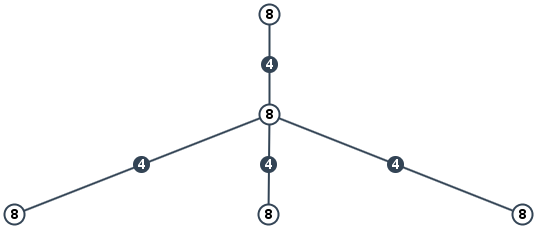
\includegraphics[width=0.49\textwidth]{bilder/abb1.png}} 
	\hfill
	\subfigure[eine Kante wurde auf Gewicht 1 geduziert, alle anderen haben weiterhin Gewicht 4. Alle Knoten benötigen trotzdem mindestens 8 Agenten.]{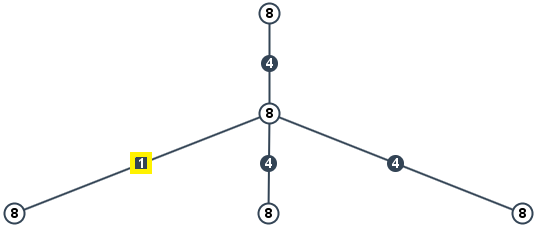
\includegraphics[width=0.49\textwidth]{bilder/abb2.png}} 
	\caption{Beispiel, dass Verringerung auf einer Kante nicht zu einer Verringerung der notwendigen Agenten führen muss} 
\end{figure} 

TODO:\\
//überlegung: woran sieht man, ob man die Agentenanzahl verringern kann?\\
//algorithmus angeben, welche kante ausgesucht wird?\\

\subsection{Potenzial verteilen mit k > 1}
	
	\section{Kooperative Gruppe}
	// wird das behandelt???
	
	\section{Fazit}
	
	
\end{document}
